\section{Parser Generator}\label{sec:parser}
In this section, we explain how to automatically generate JavaScript
parsers from a given ECMAScript.

\subsection{\( \bnfes \): Grammar for ECMAScript}
ECMAScript describes the JavaScript syntax using an
extension of the BNF notation.  We formally define the notation and
dub it \( \bnfes \).  It consists of a number of \textit{productions}
with the following form:
\[
  \NT{A}(\param_1, \cdots, \param_k) ::=
  (\cond_1 \Rightarrow)^? \rhs_1 \mid
  \cdots \mid
  (\cond_n \Rightarrow)^? \rhs_n
\]
The left-hand side of $::=$ represents a parametric non-terminal \( \NT{A} \)
with multiple boolean parameters \( \param_1, \cdots, \param_k \).
If a non-terminal takes no parameter, parentheses are omitted for brevity.
A production has multiple alternatives separated by $\mid$ with optional conditions.
A condition \( \cond \) is either a boolean parameter \( \param \)
or its negation \( ! \param \).  An alternative \( \rhs \) is a sequence
of symbols, where a symbol \( \symb \) is one of the following:
\begin{itemize}[leftmargin=0.5cm]
\item \( \epsilon \): the empty sequence, which passes without any conditions
\item \( \T{a} \): a terminal, which is any token
\item \( \NT{A}(\argument_1, \cdots, \argument_k) \): a non-terminal,
which takes multiple arguments where each argument \( \argument_i \) is
either a boolean value \( \kwt \) or \( \kwf \), or a parameter \( \param_i \)
\item \( \symb? \): option, which is the same with \( \symb \mid \epsilon \)
\item \( +\symb \) (\( -\symb \)) : positive (negative) lookahead,
which checks whether \( \symb \) succeeds (fails) and
\textit{never consumes any input}
\item \( \symb \butnot \symb' \): exclusion, which
first checks whether \( \symb \) succeeds
and then checks whether the parsing result does not correspond to \( \symb' \)
\item \( \nolt \): no line-terminator, which is a special symbol
that restricts the white spaces between two different symbols
\end{itemize}
For example, consider the following production:
\[
  \NT{A}(\param) ::= \param \Rightarrow \T{a}
  \mid \; !\param \Rightarrow \T{b}
  \mid  \T{c}
\]
Then, \( \NT{A}(\kwt) \) means \( \T{a} \mid \T{c} \)
and \( \NT{A}(\kwf) \) means \( \T{b} \mid \T{c} \).

\subsection{Lookahead Parsers}
To support \( \bnfes \) correctly, we propose a recursive descent
parser generator that handles both backtracking and lookahead tokens.

\smallskip

\textbf{Approach.} 
Our goal is to automatically generate a JavaScript parser from a given
ECMAScript grammar written in \( \bnfes \).  Among various parser
generators, we chose Scala parser combinators defined in
\textit{Parsing Expression Grammar (PEG)}~\cite{peg}.
PEG is a top-down (LL-style) recursive descent parser with
\textit{backtracking}.  It visits each alternative of a production in
order and backtracks to its previous production when parsing fails.
We chose Scala parser combinators because of the following reasons:

\begin{itemize}[leftmargin=0.5cm]
\item \textbf{Context-sensitive tokens:} ECMAScript tokens are
context-sensitive because of JavaScript regular expressions and
template strings.  For example, \( \code{/x/g} \) could be a single
regular expression token or four tokens that represent division by
variables \( \code{x} \) and \( \code{g} \) depending on enclosing
contexts.  Thus, lexers should be evaluated during parsing not before
parsing.  Since Scala parser combinators also treat lexers as parsers,
we can use appropriate lexers depending on parsing contexts.
\item \textbf{\( \bnfes \) symbols:} PEG can represent \( \bnfes \)
symbols intuitively as we explain in Section~\ref{sec:convert-bnfes}.
\item \textbf{Multiple starting non-terminals:} Since ECMAScript 6,
both scripts and modules serve as starting points of parsers.  Scala
parser combinators allow to use any non-terminals as parsers.
\item \textbf{Parsing at run-time:} JavaScript supports the \( \code{eval} \)
function that parses a given JavaScript string value to code and
evaluates it.  Moreover, syntax-directed abstract algorithms use special
phrases like ``the \( N \) that is \textit{covered by} \( P \),'' which
means that a generalized parser parses the syntax tree \( P \) because
finding a specific parser to correctly parse it requires its
evaluation context.  When a JavaScript interpreter encounters such a
phrase, it decides a specific parser to \( N \) and parses the given
syntax tree \( P \) with the non-terminal \( N \) again at run time.
\end{itemize}

\smallskip

\textbf{Problem: Prioritized Choices.} While PEG provides all the
features we discussed so far, it has one fundamental problem:
\textit{prioritized choices}.  In PEG, the pipe \( \mid \) operator
denotes a prioritized choice; even when multiple alternatives are
applicable, PEG always picks the first success alternative.  However,
some non-terminals of the ECMAScript grammar accept multiple
alternatives for given input strings.  For example, consider the
following simplified grammar of the JavaScript expressions:
\[
  \begin{array}{r@{~}c@{~}l}
    \NT{A} &::=& \NT{T} \T{;} \mid \NT{A} \; \T{+} \; \NT{T} \T{;} \\
    \NT{T} &::=& \T{a} \mid \T{a} \T{(} \T{b} \T{)}\\
  \end{array}
\]
The non-terminal \( \NT{T} \) should accept both alternatives for
\( \code{a(b);} \), but PEG-based parsers fail to parse it because the
first alternative \( \T{a} \) succeeds first and the second alternative
\( \T{a} \T{(} \T{b} \T{)} \) is not reachable.  A simple solution is
to change the order of alternatives like \( \NT{T} ::= \T{a} \T{(} \T{b} \T{)} \mid \T{a} \),
but ensuring correct order is not trivial because it requires
calculation of their inclusion relationship.  Moreover, simple
reordering does not work for some productions:
\[
  \begin{array}{r@{~}c@{~}l}
    \NT{A} &::=& \NT{B} \; \T{b}\\
    \NT{B} &::=& \T{a} \mid \T{a} \; \T{b}\\
  \end{array}
\]
The non-terminal \( \NT{A} \) should successfully parse two strings
\( \code{ab} \) and \( \code{abb} \),  but it accepts only \( \code{ab} \),
and it accepts only \( \code{abb} \) if \( \NT{B} ::= \T{a} \; \T{b} \mid \T{a} \).
Hence, we should re-structure the above rules to accept both strings
in traditional PEG grammars.

\begin{figure}[t]
\centering
\small
\[
  \begin{array}{l@{~}c@{~}l}
    \rhsfirst{\symb_1 \cdots \symb_n} &=& \symbfirst{\symb_1} \firstplus
    \symbfirst{\symb_2 \cdots \symb_n}\\
    && \text{where} \; x \firstplus y = \left\{
    \begin{array}{ll}
      x \cup y & \text{if} \; \emptyfirst \in x\\
      x & \text{otherwise}\\
    \end{array}
    \right.\\
    \symbfirst{\epsilon} &=& \{ \emptyfirst \}\\
    \symbfirst{\T{a}} &=& \{ \T{a} \} \\
    \symbfirst{\NT{A}(\argument_1, \cdots, \argument_k)} &=&
    \rhsfirst{\rhs_1} \cup \cdots \cup \rhsfirst{\rhs_n}\\
    && \text{where} \; \NT{A}(\argument_1, \cdots, \argument_k) =
    \rhs_1 \mid \cdots \mid \rhs_n\\
    \symbfirst{\symb?} &=& \symbfirst{\symb} \cup \{ \emptyfirst \}\\
    \symbfirst{+\symb} &=& \symbfirst{\symb}\\
    \symbfirst{-\symb} &=& \{ \emptyfirst \}\\
    \symbfirst{\symb \butnot \symb'} &=& \symbfirst{\symb}\\
    \symbfirst{\nolt} &=& \{ \emptyfirst \}
  \end{array}
\]
\vspace*{-1em}
\caption{Over-approximated first tokens of \( \bnfes \) symbols}
\label{fig:first-tokens}
\end{figure}

\smallskip

\textbf{Solution: Lookahead Tokens.}
To alleviate the problem, we propose \textit{lookahead parsers},
which are recursive descent parsers extended with backtracking and
\textit{lookahead tokens}.  They keep track of the next possible
tokens by statically calculating first tokens of each symbol using the
algorithm in Figure~\ref{fig:first-tokens}.  For example, the
following steps explain how to utilize lookahead tokens during parsing
with the input \( \code{a(b);} \):
\begin{center}
  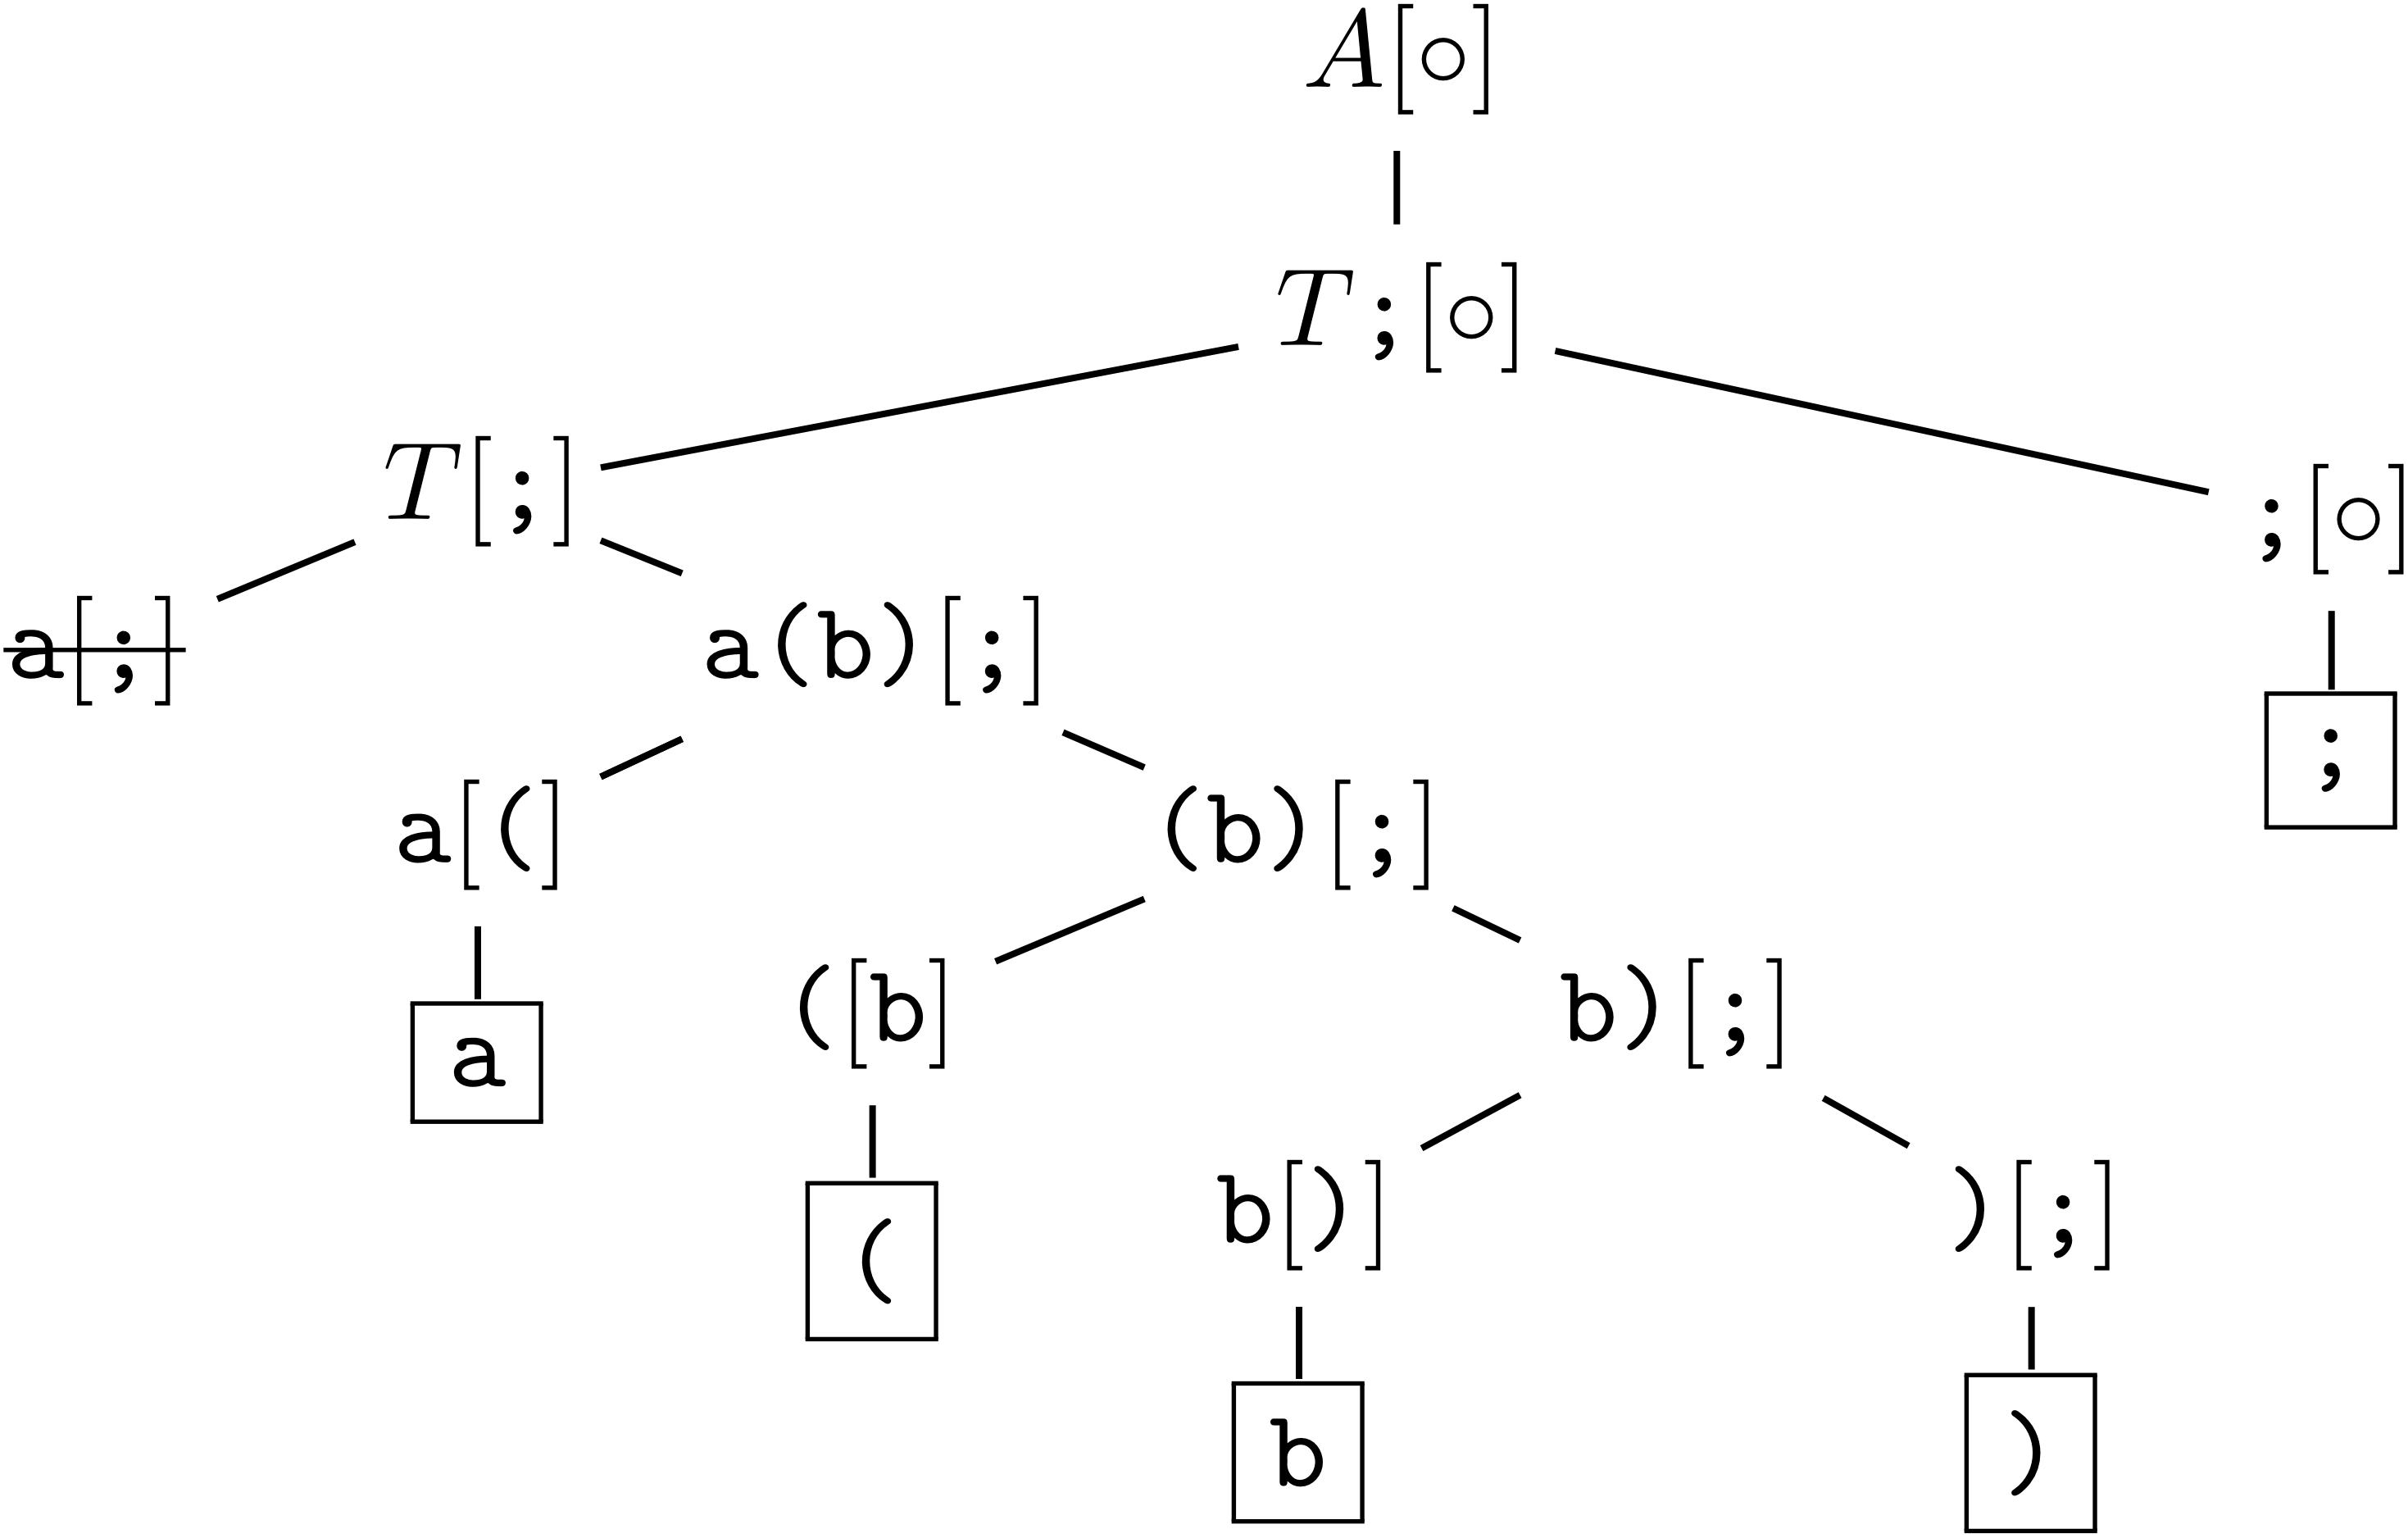
\includegraphics[width=0.3\textwidth]{img/laparser.png}
\end{center}
Each node \( \symb^*[\la] \) denotes a sequence of symbols \( \symb^* \)
with a set of lookahead tokens \( \la \).  The parsing process follows
a pre-order traversal.  It starts from the starting non-terminal \( \NT{A} \)
with the special lookahead \( \emptyfirst \), which denotes the end of
inputs.  Then, it visits the first alternative \( \NT{T} \T{;} \) with
the same lookahead.  Each symbol is visited with its corresponding
lookahead, which is the first tokens of the right next symbol.
For example, for the symbol \( \NT{T} \), the next symbol is \( \T{;} \)
and its first token is itself.  Thus, the parser visits \( \NT{T} \)
with the lookahead \( \T{;} \).  The most important point here
is the first alternative \( \T{a} \) of the
non-terminal \( \NT{T} \).  The parser visits it with the lookahead \( \T{;} \)
but the next token of the input string \( \code{a(b);} \) is \( \code{(} \)
rather than \( \code{;} \).  Hence, it fails to parse the input string
even though the current token is the same with the terminal \( \T{a} \).
Therefore, the parser can visit the next alternative \( \T{a}\T{(}\T{b}\T{)} \)
and successfully parses the input \( \code{a(b);} \).

\begin{figure}[t]
\centering
\small
\[
  \begin{array}{l@{~}c@{~}l}
    (\symb_1 \cdots \symb_n)[\la] &=&
    \symb_1[\symbfirst{\symb_2 \cdots \symb_n} \firstplus \la] \;
    (\symb_1 \cdots \symb_n)[\la]\\
    \epsilon[\la] &=& +\getlap{\la}\\
    \T{a}[\la] &=& \T{a} \; +\getlap{\la} \\
    \NT{A}(\argument_1, \cdots, \argument_k)[\la] &=&
    \rhs_1[\la] \mid \cdots \mid \rhs_n[\la]\\
    && \text{where} \; \NT{A}(\argument_1, \cdots, \argument_k) =
    \rhs_1 \mid \cdots \mid \rhs_n\\

    \symb?[\la] &=& \symb[\la] \mid \epsilon[\la]\\
    (\pm\symb)[\la] &=& \pm(\symb[\la]) \\
    (\symb \butnot \symb')[\la] &=& \symb[\la] \butnot \symb'\\
    \nolt &=& \nolt \; +\getlap{\la}\\
  \end{array}
\]
\vspace*{-1em}
\caption{Formal semantics of lookahead parsers}
\label{fig:laparser}
\vspace*{-1em}
\end{figure}

We formally define the semantics of lookahead parsers in Figure~\ref{fig:laparser}.
The helper function \( \getlap{\la} \) generates a parser by combining all
tokens in the lookahead \( \la \) using prioritized choices.
In this case, the order does not change the semantics of lookahead parsers
because \( \getlap{\la} \) just checks the existence of a given token.

\subsection{Implementation}\label{sec:convert-bnfes}
We implemented lookahead parsers by extending Scala parser combinators
with two functions corresponding to Figure~\ref{fig:first-tokens} and
Figure~\ref{fig:laparser}.

\smallskip

\textbf{AST Generation.}
We first automatically generate ASTs as Scala case classes from a
given \( \bnfes \) grammar.  Because lexical grammars do not affect
the ECMAScript semantics, we represent them as string values.
For parser grammars, we automatically synthesize a Scala file that has
classes of syntax trees.  For each production \(
  \NT{A}(\param_1, \cdots, \param_k) ::=
  (\cond_1 \Rightarrow)^? \rhs_1 \mid
  \cdots \mid
  (\cond_n \Rightarrow)^? \rhs_n
\), the AST generator defines the \( \code{A} \) trait and multiple
subclasses \( \code{A}_i \) of \( \code{A} \) for \(0 \le i \le n-1\)
that represents its alternatives.  Each class \( \code{A}_i \) has
non-terminals in its corresponding alternative as its fields.
For instance, the \( ArrayLiteral \) production in Figure~\ref{fig:array-literal}
gets automatically translated to the following Scala classes:
\begin{lstlisting}[style=smallScalastyle]
trait ArrayLiteral extends AST
case class ArrayLiteral0(x1: Option[Elision])
case class ArrayLiteral1(x1: ElementList)
case class ArrayLiteral2(x1: ElementList, x3: Option[Elision])
\end{lstlisting}

\smallskip

\textbf{Parser Generation.}
The next step is to automatically extract parsers from the given \(
\bnfes \) grammar.  The conversion from \( \bnfes \) symbols into
Scala code is as follows:
\[
\small
  \begin{array}{ccc}
%    \bnfes \; \text{symbols} &\Rightarrow& \text{Scala codes}\\\hline
    \epsilon &\Rightarrow& \scode{MATCH}\\
    \T{a} &\Rightarrow& \scode{"a"}\\
    \NT{A}(\argument_1, \cdots, \argument_n) &\Rightarrow& \scode{A(a1, .. , an)}\\
    \symb? &\Rightarrow& \scode{opt(s)}\\
    \pm\symb &\Rightarrow& \pm\scode{\symb} \\
    \symb \butnot \symb' &\Rightarrow& \scode{s\textbackslash s'}\\
    \nolt &\Rightarrow& \scode{NoLineTerminator}\\
  \end{array}
\]
where \( \code{MATCH} \) denotes the empty sequence of lookahead parsers.
Each string literal gets implicitly converted to a lookahead parser via
Scala implicit conversion.  The \( \code{opt(s)} \) function is the
same with \( \code{s | MATCH} \).  We also define the \( \code{\textbackslash} \) 
operator between parsers to support exclusive parsers.
Finally, we provide the \( \code{NoLineTerminator} \) parser, which uses
the white space parsers to check the existence of line terminators.
Our approach can support such a parser because we also automatically
generate lexers not only parsers of the ECMAScript syntax.  Then, the 
automatically synthesized parser from the production \textit{ArrayLiteral}
in Figure~\ref{fig:array-literal}(a) is the one in Figure~\ref{fig:array-literal}(b).

We support the automatic semicolon insertion algorithm, which
is the most distinctive parsing feature in ECMAScript.  We extended
our parser implementation to keep track of the right-most position
that fails to be parsed in a given input.  In ECMAScript, the token at that
position is defined as an \textit{offending token} and the automatic
semicolon insertion algorithm is defined with such tokens.  The
algorithm is simple when we already have the positions of offending
tokens.  Thus, we just manually supported them by following the rules
in ES10.  In addition, the rules rarely change; since
ES5.1 written in 2011, only one sub-rule was added.

\smallskip

\textbf{Discussion.}
While implementing lookahead parsers in Scala, we resolved two issues.

First, one of the critical weak points of recursive descent parsing
with backtracking is its performance.  To support backtracking, it
requires exponential time relative to the input size.  Luckily, Ford
et al~\cite{packrat} proposed Packrat parsing that provides linear 
time complexity using memoization.  By treating each parser as a
function from the current input position to a parsing result, it just
memoizes each parser using input positions, which dramatically reduces
redundant parsing trials.  In a similar way, we treat each lookahead
parser as a function from a pair of lookahead tokens and input
positions to a parsing result.

The second issue is that recursive descent parsers do not support left
recursion in grammars.  If a grammar has a left recursion, its parser
falls into an infinite loop.  To resolve this problem, Warth et
al~\cite{packrat-lr} proposed a mechanism to support not only direct
left recursion but also indirect one in Packrat parsing.  While we can
adopt the mechanism, we found that the ES10 syntax does not
use indirect left recursion.  Thus, we decided to just remove direct
left recursion by defining sub productions.
